\documentclass{beamer}

\title{Simon Fraser University \\ Pension Valuation \\ 
Acma 475}
\author{Phoebe Zhang, Nathan Esau, Layla Trummer, Albee Hong, Jonathan Royalty, Tom Dodge}
\date{November 25, 2014}

\usepackage{slides}

\begin{document}

\begin{frame}
\titlepage
\end{frame}

\begin{frame}{Agenda}
\tableofcontents
\end{frame}

\begin{frame}{Valuation Provisions}

\section{Valuation provisions}

\textbf{Plan provisions}
\begin{itemize}
\item 1.3\% of FAE up to FAYMPE + 2\% of FAE over FAYMPE
\item Earliest Retirement Age 55
\begin{itemize}
\item Normal Retirement Age 65
\end{itemize}
\item PUC Method
\begin{itemize}
\item Includes salary projection
\end{itemize}
\end{itemize}

\textbf{Solvency provisions}

\begin{itemize}
\item TUC method
\begin{itemize}
\item No salary projection
\end{itemize}
\item Retirement age 55
\end{itemize}

\end{frame}

\begin{frame}{2012 Going--Concern and Solvency Results}

\section{Valuation Results}

\begin{table}[ht]
\def\arraystretch{1.2}
\begin{tabular}{l r r}
\hline
& Going-concern & Solvency \\ \hline
Asset & 9,571,300  & 9,271,300 \\
Liability & & \\
\hspace{2mm} Active & 8,311,200 & 9,019,200 \\ 
\hspace{2mm} Deferred & 286,000 & 417,100 \\
\hspace{2mm} Pensioner  & 1,324,400 & 1,566,400 \\
\hspace{2mm} Total & 9,921,600 & 11,002,700 \\ \hline
Surplus / Deficit & (350,300) & (1,731,400) \\ \hline
\end{tabular}
\end{table}

\end{frame}

\begin{frame}{2013 Going--Concern and Solvency Results}

\begin{table}[ht]
\def\arraystretch{1.2}
\begin{tabular}{l r r}
\hline 
& Going--Concern & Solvency \\ \hline
Asset & 10,711,300 & 10,386,300 \\ 
Liability & & \\
\hspace{2mm} Active & 6,721,500 \\ 
\hspace{2mm} Deferred & 378,200 & 497,800 \\ 
\hspace{2mm} Pensioner & 3,271,700 & 3,676,500 \\ 
\hspace{2mm} Total & 10,011,100 & 10,895,800 \\ \hline
Surplus / Deficit & 700,200 & (509,500) \\ \hline 
\end{tabular}
\end{table}

\end{frame}

\begin{frame}{2013 Plan Membership and Liabilities by Membership Group} 

\begin{itemize}
\item Total Membership Count = 61
\end{itemize}

\begin{table}[ht]
\begin{tabular}{l r r}
\hline
& Membership & Liabilities \\ \hline
Deferred  & 10\% & 4\% \\
Pensioners & 23\% & 33\% \\
Active & 67\% & 63\% \\ \hline
\end{tabular}
\end{table}

\end{frame}

\begin{frame}{Experience Gain / Loss}

\section{2013 Going-Concern Gain and Loss}

\subsection{Experience}

\begin{figure}
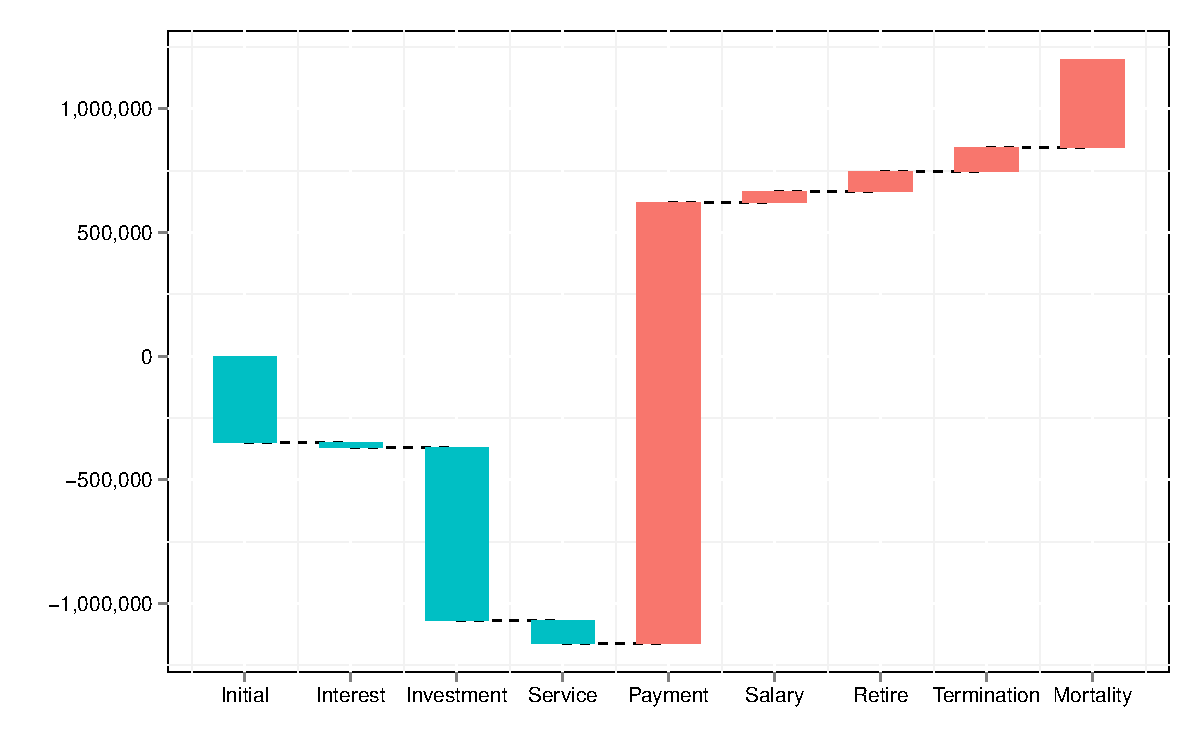
\includegraphics[width=1.0\textwidth]{waterfall}
\end{figure}

\end{frame}

\begin{frame}{Experience Gain / Loss}

\begin{itemize}
\item Investment experience was much lower than expected
\begin{itemize}
\item We expected $+5\%$ return and actual return was -1.8\%
\end{itemize}
\item Interest rates were lower than expected
\item 2013 Salaries were lower than expected
\item More plan members retired than expected
\item More plan members terminated than expected
\item Mortality was higher than expected
\item This experience resulted in changing some of our assumptions for this valuation
\end{itemize}

\end{frame}

\begin{frame}{2012 vs 2013 Assumptions}

\subsection{Change in Provisions and Assumptions}

\begin{table}[ht]
\begin{tabular}{l r r}
\hline
& Dec 31, 2013 & Dec 31, 2012 \\ \hline
Discount Rate & 4.75\% & 5\% \\
Salary Scale & 4\% & 4.25\% \\
Mortality & UP94 (to 2020) & UP94 (to 2015) \\
Retirement age & 60 & 65 \\ 
FAE / FAYMPE & 3 & 5 \\
ERR & 3\% per year & Actuarial Equivalent \\ \hline
\end{tabular}
\end{table}

\end{frame}

\begin{frame}{Assumption Gain / Loss}

\begin{figure}
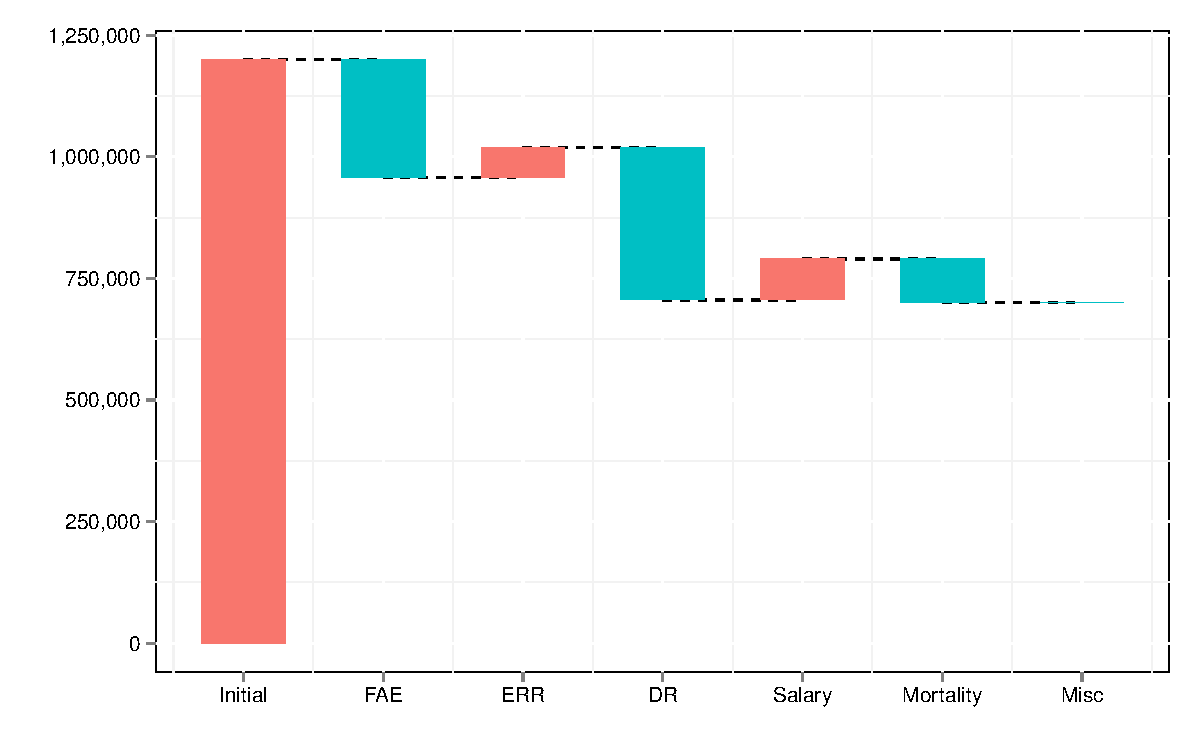
\includegraphics[width=1.0\textwidth]{waterfall2}
\end{figure}

\end{frame}

\begin{frame}{Summarized Gain / Loss}

\begin{table}[ht]
\begin{tabular}{l c c c c}
\hline
& Active & Deferred & Pensioner & Overall \\ \hline
FAE & Loss & -- & -- & Loss \\
ERR & Gain & Loss & -- & Gain \\
Discount rate & Loss & Loss & Loss & Loss \\ 
Salary Scale & Gain & -- & -- & Gain \\ 
Mortality & Loss & Loss  & Loss & Loss \\ \hline
\end{tabular}
\end{table}

\end{frame}

\begin{frame}{Assumption Gain / Loss Order of Changes}

\begin{enumerate}
\item Form (Final Average Earnings Period)
\item Retirement Age and Early Retirement Reduction
\item Salary Gain
\item Mortality Assumption
\item Discount Rate
\end{enumerate}

\end{frame}

\begin{frame}{Pension Formula: FAE5 to FAE3}

\begin{itemize}
\item Both salary and YMPE year range were changed
\item FAE3 is more favourable to plan members because salaries are increasing with age
\item FAYMPE3 is less favourable to plan members because the pension limit is higher
\end{itemize}

\medskip
\qquad\textbf{Loss}

\end{frame}

\begin{frame}{Early Retirement Reduction: Actuarial equivalent to percentage}

\begin{itemize}
\item Changed to 3\% reduction per year
\item Affects both active and deferred members
\item Favourable to plan members
\begin{itemize}
\item Actuarial equivalent is approximately 6\%
\end{itemize}
\end{itemize}

\medskip
\qquad\textbf{Loss}

\end{frame}

\begin{frame}{Retirement Age: Age 65 to 60}

\begin{itemize}
\item The ERR change will encourage plan members to retire earlier
\item Assumption change is favourable to company because final salaries and service are lower
\begin{itemize}
\item Offsets the Loss from the ERR change for going-concern valuation
\end{itemize}
\item No impact on solvency
\end{itemize}

\medskip
\qquad\textbf{Gain}

\end{frame}

\begin{frame}{Mortality: 2015 Projection to 2020 projection}

\begin{itemize}
\item Assume lower mortality over time
\item Increases company's liability on all plan members
\item Reflects improving medical care and life expectancy
\end{itemize}

\medskip
\qquad\textbf{Loss}

\end{frame}

\begin{frame}{Salary increase: 4.25\% to 4\%}

\begin{itemize}
\item Lower salary scale is favourable to the plan because it lowers liability
\item Reflects slower than expected economic recovery
\item Reflects experience gain for salary changes
\end{itemize}

\medskip
\qquad\textbf{Gain}

\end{frame}

\begin{frame}{Discount rate: 5\% to 4.75\%}

\begin{itemize}
\item Reflects slower than expected economic recovery
\item Reflects experience loss for interest rate
\item Accounts for largest impact on liabilities
\end{itemize}

\medskip
\qquad\textbf{Loss}

\end{frame}

\begin{frame}{Discount rate sensitivity}

\section{Sensitivity Impact}

\begin{table}[ht]
\begin{tabular}{l r r r}
\hline
& DR & DR - 1\% & $\Delta$ Liability \\ \hline
Going-concern & 4.75\% & 3.75\% & 1,429,183 \\
Solvency \\
\hspace{2mm} CV & 3.25\% & 2.25 & 618,900 \\
\hspace{2mm} AP & 3.50\% & 2.50\% & 854,500 \\
\hspace{2mm} Total & -- & -- & 1,473,400 \\ \hline
\end{tabular}
\end{table}

\end{frame}

\begin{frame}{2014 ER Contributions}

\section{Recommendations}

\begin{table}[ht]
\begin{tabular}{l r}
Employer Contributions & 230,700 \\
Expected 2014 Salary & 1,646,000 \\
Employer Contributions \% & 14.0\%
\end{tabular}
\end{table}

\end{frame}

\begin{frame}{Funding Recommendations}

\begin{table}[ht]
\begin{tabular}{l r r}
\hline
& Minimum & Maximum \\ \hline
Employer Contributions & 230,700 & 230,700 \\
Solvency Special Payment & 109,300 & 509,500 \\
Total Payment & 340,000 & 740,200 \\ \hline
\end{tabular}
\end{table}

\end{frame}

\end{document}